\documentclass[tikz]{standalone}
\usetikzlibrary{patterns}
\usetikzlibrary{arrows}
\usetikzlibrary{decorations.shapes,decorations.markings,decorations.pathreplacing}

\tikzset{
    set arrow inside/.code={\pgfqkeys{/tikz/arrow inside}{#1}},
    set arrow inside={end/.initial=>, opt/.initial=},
    /pgf/decoration/Mark/.style={
        mark/.expanded=at position #1 with
        {
            \noexpand\arrow[\pgfkeysvalueof{/tikz/arrow inside/opt}]{\pgfkeysvalueof{/tikz/arrow inside/end}}
        }
    },
    arrow inside/.style 2 args={
        set arrow inside={#1},
        postaction={
            decorate,decoration={
                markings,Mark/.list={#2}
            }
        }
    },
}
\begin{document}
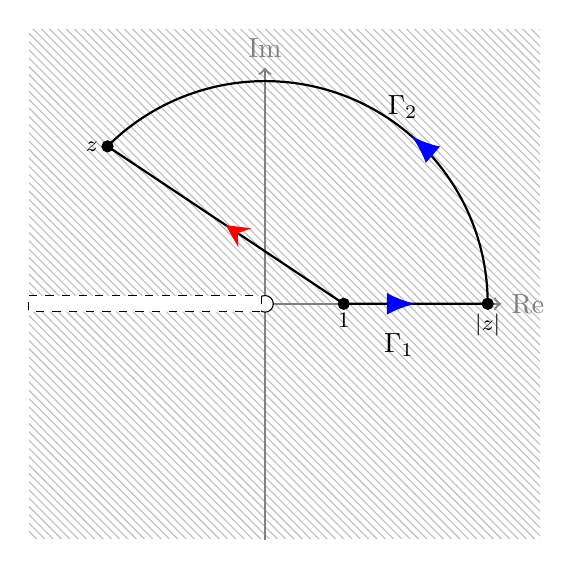
\begin{tikzpicture}
\draw[pattern=north west lines,pattern color=gray!50,draw=white] (-3,-3) -- (-3,3.5) -- (3.5,3.5) -- (3.5,-3) -- (-3,-3);
\draw[->,thick,gray] (-3,0) -- (3,0) node[right]{$\mathrm{Re}$};
\draw[->,thick,gray] (0,-3) -- (0,3) node[above]{$\mathrm{Im}$};
\draw[fill=white] (0,0) circle (3pt);
\draw[fill=white,dashed] (-3,0.1) -- (-0.05,0.1) -- (-0.05,-0.1) -- (-3,-0.1) -- (-3,0.1);
\draw[fill] (1,0) circle (2pt) node[below,font=\footnotesize]{$1$};
\draw[fill] (-2,2) circle (2pt) node[left,font=\footnotesize]{$z$};
\draw[thick] (1,0) -- (-2,2) [arrow inside={end=stealth,opt={red,scale=2}}{0.5}];
\draw (1.7,-0.25) node[below] {$\Gamma_1$} ;
\draw (1.75,2.5) node {$\Gamma_2$};
\draw[fill] ({2*sqrt(2)},0) circle (2pt) node[below,font=\footnotesize]{$|z|$};
\draw[thick] (1,0) -- ({2*sqrt(2)},0) arc(0:135:{2*sqrt(2)}) [arrow inside={end=latex,opt={blue,scale=2}}{0.5}];
\draw[thick] (1,0) -- ({2*sqrt(2)},0) [arrow inside={end=latex,opt={blue,scale=2}}{0.5}];
\end{tikzpicture}
\end{document}